\documentclass{article}
\usepackage{tikz}
\begin{document}
%we are working on
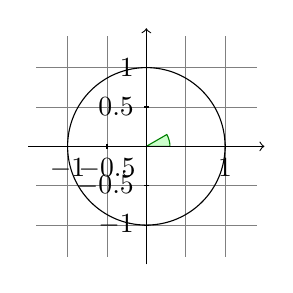
\begin{tikzpicture}
	%\clip (-0.6,-0.2) rectangle (0.6,1.51);
	\draw[step=.5cm,help lines] (-1.4,-1.4) grid (1.4,1.4);
	\filldraw[fill=green!20,draw=green!50!black]
	(0,0) -- (3mm,0mm) arc (0:30:3mm) -- cycle;
	\draw[->] (-1.5,0) -- (1.5,0);   \draw[->] (0,-1.5) -- (0,1.5);
	\draw (0,0) circle (1cm);
	\foreach \x in {-1,-0.5,1}
	\draw (\x cm,1pt) -- (\x cm,-1pt) node[anchor=north] {$\x$};
	\foreach \y in {-1,-0.5,0.5,1}
	\draw (1pt,\y cm) -- (-1pt,\y cm) node[anchor=east] {$\y$};
\end{tikzpicture}
\end{document}